\documentclass{article}
\usepackage[utf8]{inputenc}
\usepackage[T1]{fontenc}
\usepackage[french]{babel}
\usepackage{graphicx}
\usepackage{hyperref}
\usepackage{amsmath}
\usepackage{listings}
\usepackage{geometry}
\geometry{margin=1in}

\begin{document}

\title{Système de Base de Données pour le Site de Préférences Vidéo}
\author{Projet de Base de Données}
\date{\today}

\maketitle

\tableofcontents
\newpage

\section{Aperçu du Projet}

L'objectif de ce projet est de concevoir et d'implémenter un système de base de données robuste pour un site de replay vidéo qui gère les inscriptions des utilisateurs, les détails des vidéos, l'historique de visionnage et les suggestions de vidéos personnalisées. La plateforme permettra aux utilisateurs d'explorer des vidéos par catégories, de suivre leurs favoris et de recevoir des recommandations personnalisées basées sur la popularité des vidéos. La base de données gérera également le cycle de vie des vidéos, y compris l'archivage des contenus plus anciens.

\section{Objectifs}

\begin{enumerate}
    \item Développer une base de données relationnelle pour gérer :
    \begin{itemize}
        \item \textbf{Informations utilisateur} : Inscription, identifiants de connexion, détails du profil et préférences.
        \item \textbf{Détails des vidéos} : Métadonnées, disponibilité, catégorisation et cycle de vie.
        \item \textbf{Activité utilisateur} : Historique de visionnage, favoris et abonnements.
        \item \textbf{Suggestions} : Recommandations personnalisées basées sur la popularité récente des vidéos.
    \end{itemize}
    \item Assurer que la base de données puisse supporter des fonctionnalités telles que :
    \begin{itemize}
        \item Suivi de la disponibilité des vidéos et automatisation de l'archivage après expiration de la période de visionnage.
        \item Génération de suggestions dynamiques pour les utilisateurs enregistrés.
        \item Enregistrement des interactions utilisateur pour des expériences personnalisées et des analyses historiques.
    \end{itemize}
\end{enumerate}

\section{Portée}

\subsection{Entités de la Base de Données}

\begin{itemize}
    \item \textbf{Utilisateurs} :
    \begin{itemize}
        \item \textbf{Attributs} : Identifiant, mot de passe, nom, prénom, date de naissance, email, préférences (catégories d'intérêt) et statut d'abonnement à la newsletter.
        \item \textbf{Fonctionnalités} :
        \begin{itemize}
            \item Suivre les vidéos favorites.
            \item S'abonner à des émissions pour des suggestions automatiques.
            \item Accéder à l'historique de visionnage.
        \end{itemize}
    \end{itemize}
    \item \textbf{Vidéos} :
    \begin{itemize}
        \item \textbf{Attributs} : Nom, description, durée, date de sortie, pays d'origine, support multilingue, format d'image et statut de disponibilité (actif/archivé).
        \item \textbf{Fonctionnalités} :
        \begin{itemize}
            \item Classées en catégories (par exemple, culture, cinéma).
            \item Support des émissions à plusieurs épisodes.
            \item Gestion du cycle de vie (disponibilité minimale de 7 jours, règles d'archivage).
        \end{itemize}
    \end{itemize}
    \item \textbf{Historique de Visionnage} :
    \begin{itemize}
        \item \textbf{Attributs} : ID utilisateur, ID vidéo, date de visionnage.
        \item \textbf{Fonctionnalités} :
        \begin{itemize}
            \item Maintenir un enregistrement des vidéos visionnées par chaque utilisateur.
        \end{itemize}
    \end{itemize}
    \item \textbf{Suggestions} :
    \begin{itemize}
        \item Générées en fonction de :
        \begin{itemize}
            \item Popularité au sein des catégories (nombre de visionnages au cours des deux dernières semaines).
            \item Abonnements de l'utilisateur aux émissions.
        \end{itemize}
    \end{itemize}
\end{itemize}

\subsection{Fonctionnalités Clés}

\begin{enumerate}
    \item \textbf{Gestion des Utilisateurs} :
    \begin{itemize}
        \item Permettre aux utilisateurs de créer des comptes, de se connecter et de gérer leurs préférences.
        \item Fournir l'option de s'abonner aux newsletters et à des catégories spécifiques de programmes.
    \end{itemize}
    \item \textbf{Cycle de Vie des Vidéos} :
    \begin{itemize}
        \item Archiver automatiquement les vidéos après une durée spécifique tout en garantissant au moins 7 jours de disponibilité.
    \end{itemize}
    \item \textbf{Expérience de Visionnage} :
    \begin{itemize}
        \item Permettre aux utilisateurs de marquer des vidéos comme favorites et de les afficher sur une page personnalisée.
        \item Mettre en évidence les vidéos approchant de la fin de leur disponibilité.
    \end{itemize}
    \item \textbf{Système de Recommandation} :
    \begin{itemize}
        \item Générer des suggestions basées sur la popularité des catégories au cours des deux dernières semaines.
    \end{itemize}
    \item \textbf{Analyse de Données} :
    \begin{itemize}
        \item Suivre les visionnages de vidéos et les tendances de popularité.
    \end{itemize}
\end{enumerate}

\section{Entités}

Voici un aperçu détaillé des entités et de leurs attributs associés :

\subsection{Utilisateur}

\begin{itemize}
    \item \textbf{Attributs} :
    \begin{itemize}
        \item \textbf{Identifiant} (Unique)
        \item \textbf{Mot de passe}
        \item \textbf{Prénom}
        \item \textbf{Nom}
        \item \textbf{Date de naissance}
        \item \textbf{Adresse email}
        \item \textbf{Catégories d'intérêt}
        \item \textbf{Abonnement à la newsletter hebdomadaire} (Booléen : Oui/Non)
    \end{itemize}
    \item \textbf{Relations} :
    \begin{itemize}
        \item S'abonne à des émissions (Relation Plusieurs-à-Plusieurs avec \textbf{Émission})
        \item Marque des vidéos comme favorites (Relation Plusieurs-à-Plusieurs avec \textbf{Vidéo})
        \item Possède un historique de visionnage (Relation Un-à-Plusieurs avec \textbf{Visionnage Vidéo})
    \end{itemize}
\end{itemize}

\subsection{Vidéo}

\begin{itemize}
    \item \textbf{Attributs} :
    \begin{itemize}
        \item \textbf{ID Vidéo} (Unique)
        \item \textbf{Nom}
        \item \textbf{Description}
        \item \textbf{Durée}
        \item \textbf{Date de sortie}
        \item \textbf{Pays d'origine}
        \item \textbf{Disponibilité multilingue} (Booléen : Oui/Non)
        \item \textbf{Format d'image}
        \item \textbf{Statut} (Disponible/Archivé)
    \end{itemize}
    \item \textbf{Relations} :
    \begin{itemize}
        \item Appartient à un programme (Relation Plusieurs-à-Un avec \textbf{Programme})
        \item Apparaît dans les favoris des utilisateurs (Relation Plusieurs-à-Plusieurs avec \textbf{Utilisateur})
        \item Visionnée dans l'historique des utilisateurs (Relation Un-à-Plusieurs avec \textbf{Visionnage Vidéo})
    \end{itemize}
\end{itemize}

\subsection{Programme}

\begin{itemize}
    \item \textbf{Attributs} :
    \begin{itemize}
        \item \textbf{ID Programme} (Unique)
        \item \textbf{Nom}
        \item \textbf{Catégorie} (e.g., Culture, Cinéma)
    \end{itemize}
    \item \textbf{Relations} :
    \begin{itemize}
        \item Inclut des épisodes/vidéos (Relation Un-à-Plusieurs avec \textbf{Vidéo})
    \end{itemize}
\end{itemize}

\subsection{Visionnage Vidéo}

\begin{itemize}
    \item \textbf{Attributs} :
    \begin{itemize}
        \item \textbf{ID Visionnage} (Unique)
        \item \textbf{ID Utilisateur} (Clé étrangère vers \textbf{Utilisateur})
        \item \textbf{ID Vidéo} (Clé étrangère vers \textbf{Vidéo})
        \item \textbf{Horodatage du visionnage}
    \end{itemize}
    \item \textbf{Relations} :
    \begin{itemize}
        \item Suit l'historique de visionnage de l'utilisateur (Relation Plusieurs-à-Un avec \textbf{Utilisateur})
        \item Indique quelle vidéo a été visionnée (Relation Plusieurs-à-Un avec \textbf{Vidéo})
    \end{itemize}
\end{itemize}

\subsection{Catégorie}

\begin{itemize}
    \item \textbf{Attributs} :
    \begin{itemize}
        \item \textbf{ID Catégorie} (Unique)
        \item \textbf{Nom}
    \end{itemize}
    \item \textbf{Relations} :
    \begin{itemize}
        \item Associée à des programmes (Relation Un-à-Plusieurs avec \textbf{Programme})
    \end{itemize}
\end{itemize}

\subsection{Suggestions de Visionnage}

\begin{itemize}
    \item \textbf{Attributs} :
    \begin{itemize}
        \item \textbf{ID Suggestion} (Unique)
        \item \textbf{Horodatage de génération}
        \item \textbf{Données de popularité de catégorie} (Nombre de visionnages au cours des deux dernières semaines)
    \end{itemize}
    \item \textbf{Relations} :
    \begin{itemize}
        \item Vidéos suggérées (Relation Un-à-Plusieurs avec \textbf{Vidéo})
    \end{itemize}
\end{itemize}

\section{Création de la Base de Données}

J'ai utilisé PostgreSQL 17 pour la gestion de la base de données.

\subsection{Tables SQL}

\begin{lstlisting}[language=SQL]
-- 1. Table Utilisateurs
CREATE TABLE users (
    user_id SERIAL PRIMARY KEY,
    login VARCHAR(50) UNIQUE NOT NULL,
    password VARCHAR(255) NOT NULL,
    first_name VARCHAR(50),
    last_name VARCHAR(50),
    date_of_birth DATE,
    email VARCHAR(100) UNIQUE,
    interested_categories TEXT[], -- Tableau de catégories
    newsletter_subscription BOOLEAN DEFAULT FALSE
);

-- 2. Table Catégories
CREATE TABLE categories (
    category_id SERIAL PRIMARY KEY,
    name VARCHAR(50) UNIQUE NOT NULL
);

-- 3. Table Programmes
CREATE TABLE programs (
    program_id SERIAL PRIMARY KEY,
    name VARCHAR(100) NOT NULL,
    category_id INT REFERENCES categories(category_id) ON DELETE SET NULL
);

-- 4. Table Vidéos
CREATE TABLE videos (
    video_id SERIAL PRIMARY KEY,
    name VARCHAR(100) NOT NULL,
    description TEXT,
    duration INTERVAL NOT NULL,
    release_date DATE NOT NULL,
    country_of_origin VARCHAR(50),
    multi_language_available BOOLEAN DEFAULT FALSE,
    image_format VARCHAR(50),
    status VARCHAR(10) DEFAULT 'Available', -- 'Available' ou 'Archived'
    program_id INT REFERENCES programs(program_id) ON DELETE CASCADE
);

-- 5. Table Vidéos Favorites (Relation Plusieurs-à-Plusieurs entre Utilisateurs et Vidéos)
CREATE TABLE favorite_videos (
    user_id INT REFERENCES users(user_id) ON DELETE CASCADE,
    video_id INT REFERENCES videos(video_id) ON DELETE CASCADE,
    PRIMARY KEY (user_id, video_id)
);

-- 6. Table Visionnages Vidéo
CREATE TABLE video_viewings (
    viewing_id SERIAL PRIMARY KEY,
    user_id INT REFERENCES users(user_id) ON DELETE CASCADE,
    video_id INT REFERENCES videos(video_id) ON DELETE CASCADE,
    viewing_timestamp TIMESTAMP DEFAULT CURRENT_TIMESTAMP
);

-- 7. Table Suggestions de Visionnage
CREATE TABLE viewing_suggestions (
    suggestion_id SERIAL PRIMARY KEY,
    generated_timestamp TIMESTAMP DEFAULT CURRENT_TIMESTAMP,
    category_id INT REFERENCES categories(category_id) ON DELETE CASCADE,
    video_id INT REFERENCES videos(video_id) ON DELETE CASCADE
);

-- 8. Table Programmes Abonnés (Relation Plusieurs-à-Plusieurs entre Utilisateurs et Programmes)
CREATE TABLE subscribed_programs (
    user_id INT REFERENCES users(user_id) ON DELETE CASCADE,
    program_id INT REFERENCES programs(program_id) ON DELETE CASCADE,
    PRIMARY KEY (user_id, program_id)
);
\end{lstlisting}

Après exécution, pour voir la liste des tables, j'utilise la requête suivante :

\begin{lstlisting}[language=SQL]
SELECT * FROM pg_catalog.pg_tables WHERE schemaname='public';
\end{lstlisting}

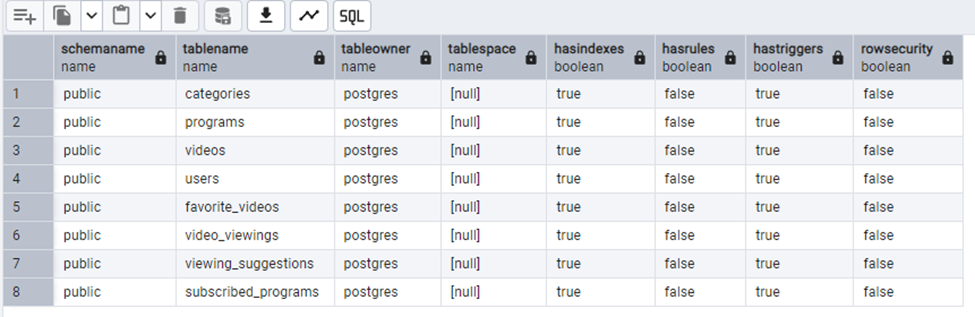
\includegraphics[width=\textwidth]{photo1.jpg}

\subsection{Modèle E/A}

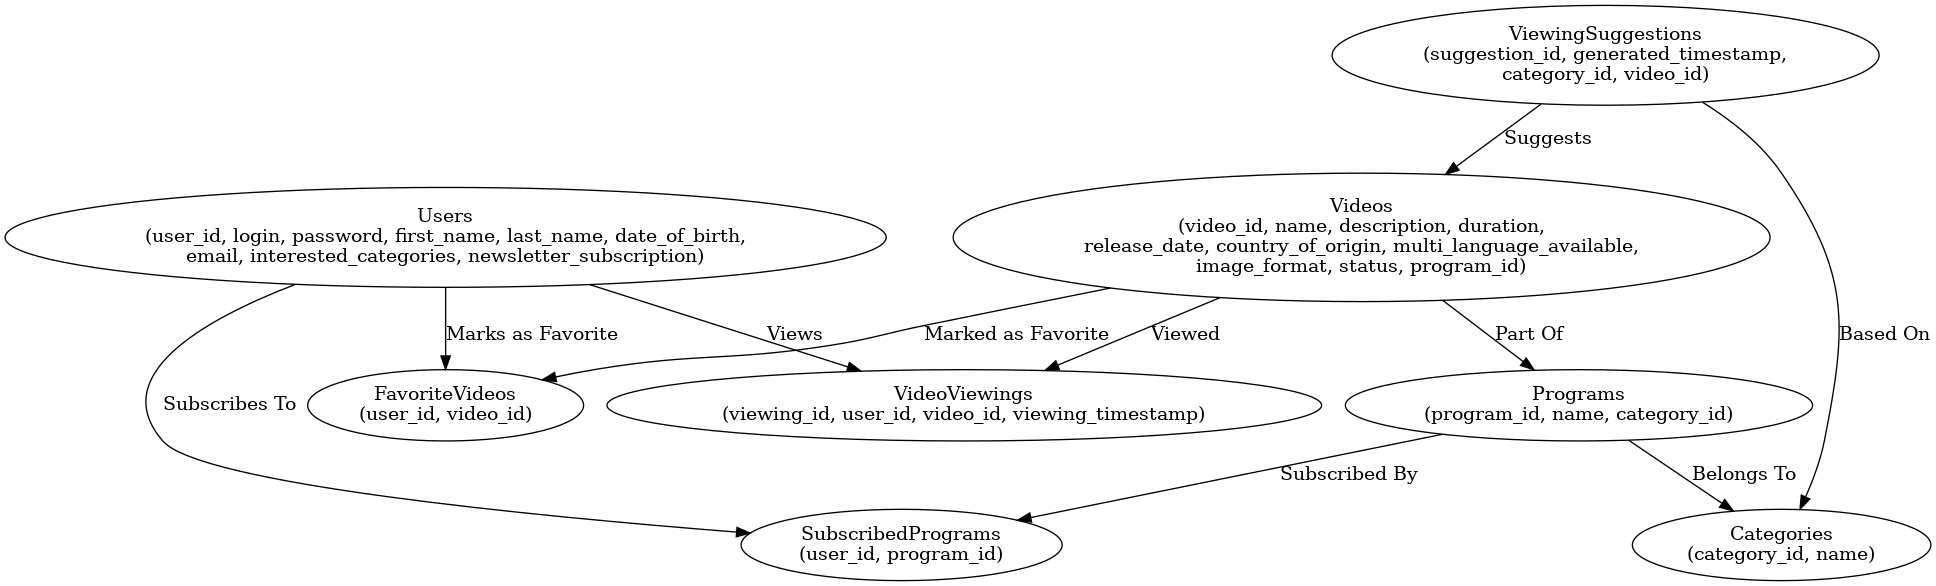
\includegraphics[width=\textwidth]{photo2.jpg}

\subsection{Modèle ERD}

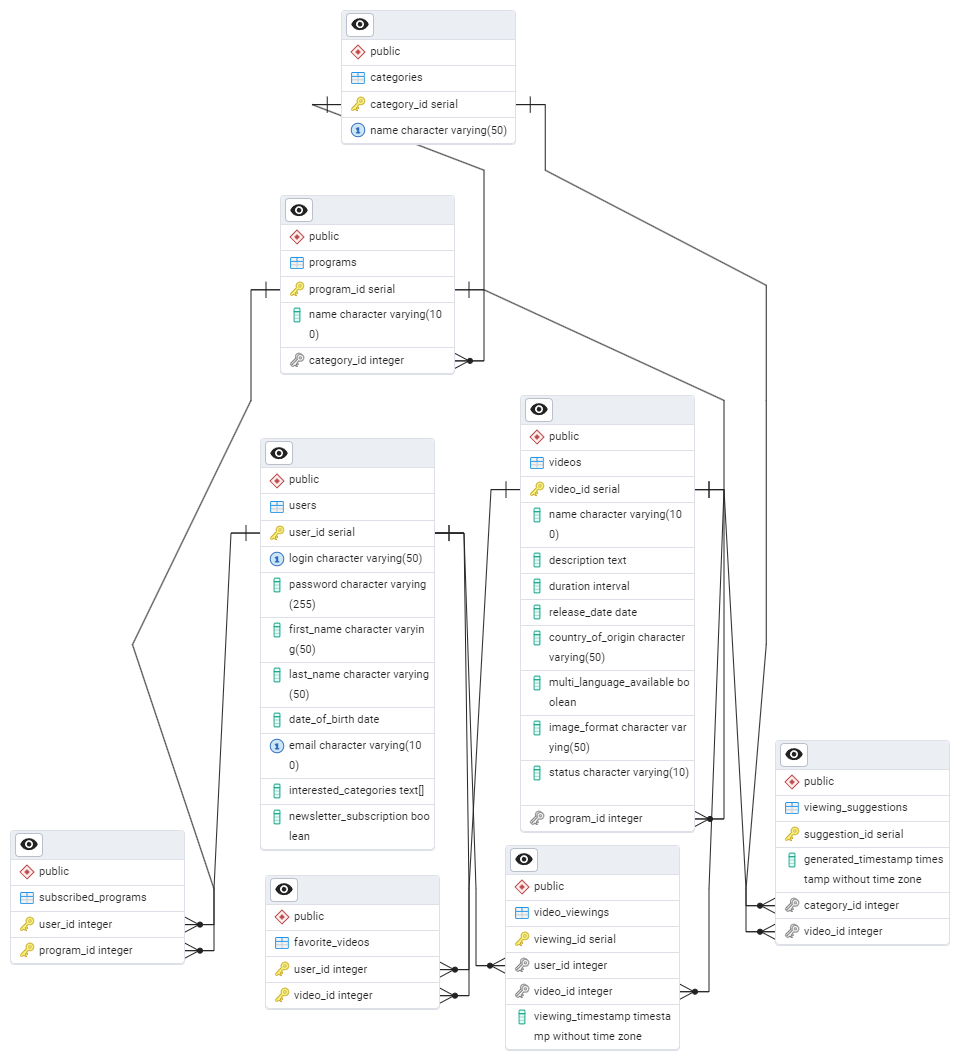
\includegraphics[width=\textwidth]{photo3.jpg}

\section{Requêtes SQL}

\subsection{Nombre de visionnages de vidéos par catégorie pour les visionnages de moins de deux semaines}

\begin{lstlisting}[language=SQL]
SELECT 
    c.name AS category_name,
    COUNT(vv.viewing_id) AS total_views
FROM 
    video_viewings vv
JOIN 
    videos v ON vv.video_id = v.video_id
JOIN 
    programs p ON v.program_id = p.program_id
JOIN 
    categories c ON p.category_id = c.category_id
WHERE 
    vv.viewing_timestamp >= NOW() - INTERVAL '14 days'
GROUP BY 
    c.name
ORDER BY 
    total_views DESC;
\end{lstlisting}

\subsection{Par utilisateur, le nombre d'abonnements, de favoris et de vidéos visionnées}

\begin{lstlisting}[language=SQL]
SELECT 
    u.user_id,
    u.first_name || ' ' || u.last_name AS user_name,
    COALESCE(subscriptions.count, 0) AS total_subscriptions,
    COALESCE(favorites.count, 0) AS total_favorites,
    COALESCE(viewings.count, 0) AS total_videos_viewed
FROM 
    users u
LEFT JOIN 
    (SELECT user_id, COUNT(*) AS count 
     FROM subscribed_programs 
     GROUP BY user_id) subscriptions 
ON u.user_id = subscriptions.user_id
LEFT JOIN 
    (SELECT user_id, COUNT(*) AS count 
     FROM favorite_videos 
     GROUP BY user_id) favorites 
ON u.user_id = favorites.user_id
LEFT JOIN 
    (SELECT user_id, COUNT(*) AS count 
     FROM video_viewings 
     GROUP BY user_id) viewings 
ON u.user_id = viewings.user_id
ORDER BY 
    u.user_id;
\end{lstlisting}

\subsection{Nombre de visionnages par des utilisateurs français et allemands, différence triée par valeur absolue}

\begin{lstlisting}[language=SQL]
ALTER TABLE users ADD COLUMN country VARCHAR(50);

SELECT 
    v.video_id,
    v.name AS video_name,
    COALESCE(french_views.count, 0) AS french_views,
    COALESCE(german_views.count, 0) AS german_views,
    ABS(COALESCE(french_views.count, 0) - COALESCE(german_views.count, 0)) AS view_difference
FROM 
    videos v
LEFT JOIN 
    (SELECT vv.video_id, COUNT(*) AS count
     FROM video_viewings vv
     JOIN users u ON vv.user_id = u.user_id
     WHERE u.country = 'France'
     GROUP BY vv.video_id) french_views 
ON v.video_id = french_views.video_id
LEFT JOIN 
    (SELECT vv.video_id, COUNT(*) AS count
     FROM video_viewings vv
     JOIN users u ON vv.user_id = u.user_id
     WHERE u.country = 'Germany'
     GROUP BY vv.video_id) german_views 
ON v.video_id = german_views.video_id
ORDER BY 
    ABS(COALESCE(french_views.count, 0) - COALESCE(german_views.count, 0)) DESC;
\end{lstlisting}

\subsection{Épisodes ayant au moins deux fois plus de visionnages que la moyenne des autres épisodes du programme}

\begin{lstlisting}[language=SQL]
SELECT 
    v.video_id,
    v.name AS episode_name,
    v.program_id,
    p.name AS program_name,
    COUNT(vv.viewing_id) AS episode_viewers
FROM 
    videos v
JOIN 
    programs p ON v.program_id = p.program_id
JOIN 
    video_viewings vv ON v.video_id = vv.video_id
GROUP BY 
    v.video_id, v.name, v.program_id, p.name
HAVING 
    COUNT(vv.viewing_id) >= 2 * (
        SELECT AVG(episode_views)
        FROM (
            SELECT 
                COUNT(vv_inner.viewing_id) AS episode_views
            FROM 
                videos v_inner
            JOIN 
                video_viewings vv_inner ON v_inner.video_id = vv_inner.video_id
            WHERE 
                v_inner.program_id = v.program_id
            GROUP BY 
                v_inner.video_id
        ) AS program_averages
    )
ORDER BY 
    episode_viewers DESC;
\end{lstlisting}

\subsection{Les 10 paires de vidéos apparaissant le plus souvent simultanément dans l'historique de visionnage des utilisateurs}

\begin{lstlisting}[language=SQL]
SELECT 
    vh1.video_id AS video_1,
    vh2.video_id AS video_2,
    COUNT(*) AS pair_count
FROM 
    video_viewings vh1
JOIN 
    video_viewings vh2 
ON 
    vh1.user_id = vh2.user_id AND vh1.video_id < vh2.video_id
GROUP BY 
    vh1.video_id, vh2.video_id
ORDER BY 
    pair_count DESC
LIMIT 10;
\end{lstlisting}

\section{Procédures et Fonctions PL/SQL}

\subsection{Fonction pour convertir les informations d'une vidéo au format JSON}

\begin{lstlisting}[language=SQL]
CREATE OR REPLACE FUNCTION get_video_json(video_id_input INT)
RETURNS JSON AS $$
DECLARE
    video_info JSON;
BEGIN
    SELECT 
        JSON_BUILD_OBJECT(
            'video_id', v.video_id,
            'name', v.name,
            'description', v.description,
            'duration', v.duration,
            'release_date', v.release_date,
            'country_of_origin', v.country_of_origin,
            'multi_language_available', v.multi_language_available,
            'image_format', v.image_format,
            'status', v.status,
            'program', JSON_BUILD_OBJECT(
                'program_id', p.program_id,
                'program_name', p.name
            )
        )
    INTO video_info
    FROM videos v
    LEFT JOIN programs p ON v.program_id = p.program_id
    WHERE v.video_id = video_id_input;

    RETURN video_info;
END;
$$ LANGUAGE plpgsql;
\end{lstlisting}

\textbf{Utilisation} :

\begin{lstlisting}[language=SQL]
SELECT get_video_json(1);
\end{lstlisting}

\subsection{Procédure pour générer le texte initial de la newsletter hebdomadaire}

\begin{lstlisting}[language=SQL]
CREATE OR REPLACE PROCEDURE generate_weekly_newsletter()
LANGUAGE plpgsql
AS $$
DECLARE
    current_week_start DATE := DATE_TRUNC('week', CURRENT_DATE);
    current_week_end DATE := current_week_start + INTERVAL '6 days';
    weekly_releases TEXT := '';
    video_record RECORD;
BEGIN
    FOR video_record IN 
        SELECT 
            name, 
            release_date, 
            description 
        FROM 
            videos 
        WHERE 
            release_date BETWEEN current_week_start AND current_week_end
    LOOP
        weekly_releases := weekly_releases || 
            '• ' || video_record.name || ' (Sortie le : ' || video_record.release_date || ') - ' || 
            video_record.description || E'\n';
    END LOOP;

    RAISE NOTICE 'Newsletter Hebdomadaire : %', 
    E'Voici les nouvelles sorties de la semaine :\n\n' || weekly_releases || 
    E'\nRestez à l\'écoute pour plus de mises à jour !';

END;
$$;
\end{lstlisting}

\textbf{Utilisation} :

\begin{lstlisting}[language=SQL]
CALL generate_weekly_newsletter();
\end{lstlisting}

\subsection{Générer la liste des vidéos populaires recommandées pour un utilisateur}

\begin{lstlisting}[language=SQL]
CREATE OR REPLACE FUNCTION recommend_videos(user_id_input INT)
RETURNS TABLE (
    video_id INT,
    video_name TEXT,
    description TEXT,
    release_date DATE,
    popularity_score INT
) AS $$
BEGIN
    RETURN QUERY
    SELECT 
        v.video_id,
        v.name AS video_name,
        v.description,
        v.release_date,
        COUNT(vv.viewing_id) AS popularity_score
    FROM 
        videos v
    JOIN 
        programs p ON v.program_id = p.program_id
    JOIN 
        categories c ON p.category_id = c.category_id
    JOIN 
        users u ON u.user_id = user_id_input
    LEFT JOIN 
        video_viewings vv ON v.video_id = vv.video_id
    WHERE 
        c.category_id = ANY(u.interested_categories)
        AND v.status = 'Available'
    GROUP BY 
        v.video_id, v.name, v.description, v.release_date
    ORDER BY 
        popularity_score DESC, v.release_date DESC
    LIMIT 10;
END;
$$ LANGUAGE plpgsql;
\end{lstlisting}

\textbf{Utilisation} :

\begin{lstlisting}[language=SQL]
SELECT * FROM recommend_videos(1);
\end{lstlisting}

\section{Déclencheurs}

\subsection{Limiter les favoris à 300 vidéos par utilisateur}

\textbf{Étape 1 : Créer la Fonction de Déclenchement}

\begin{lstlisting}[language=SQL]
CREATE OR REPLACE FUNCTION enforce_bookmark_limit()
RETURNS TRIGGER AS $$
BEGIN
    IF (
        SELECT COUNT(*) 
        FROM favorite_videos 
        WHERE user_id = NEW.user_id
    ) >= 300 THEN
        RAISE EXCEPTION 'L\'utilisateur % ne peut pas avoir plus de 300 vidéos favorites.', NEW.user_id;
    END IF;

    RETURN NEW;
END;
$$ LANGUAGE plpgsql;
\end{lstlisting}

\textbf{Étape 2 : Créer le Déclencheur}

\begin{lstlisting}[language=SQL]
CREATE TRIGGER check_bookmark_limit
BEFORE INSERT ON favorite_videos
FOR EACH ROW
EXECUTE FUNCTION enforce_bookmark_limit();
\end{lstlisting}

\textbf{Test} :

\begin{lstlisting}[language=SQL]
INSERT INTO favorite_videos (user_id, video_id)
VALUES (1, 101);
\end{lstlisting}

Si l'utilisateur a déjà 300 favoris, l'insertion échouera avec le message :

\textit{ERREUR : L'utilisateur 1 ne peut pas avoir plus de 300 vidéos favorites.}

\subsection{Archivage des vidéos supprimées}

\textbf{Étape 1 : Créer la Table d'Archive}

\begin{lstlisting}[language=SQL]
CREATE TABLE archived_videos (
    video_id INT PRIMARY KEY,
    name VARCHAR(100),
    description TEXT,
    duration INTERVAL,
    release_date DATE,
    country_of_origin VARCHAR(50),
    multi_language_available BOOLEAN,
    image_format VARCHAR(50),
    archived_at TIMESTAMP DEFAULT CURRENT_TIMESTAMP
);
\end{lstlisting}

\textbf{Étape 2 : Créer la Fonction de Déclenchement}

\begin{lstlisting}[language=SQL]
CREATE OR REPLACE FUNCTION archive_video_before_delete()
RETURNS TRIGGER AS $$
BEGIN
    INSERT INTO archived_videos (
        video_id, 
        name, 
        description, 
        duration, 
        release_date, 
        country_of_origin, 
        multi_language_available, 
        image_format
    )
    VALUES (
        OLD.video_id,
        OLD.name,
        OLD.description,
        OLD.duration,
        OLD.release_date,
        OLD.country_of_origin,
        OLD.multi_language_available,
        OLD.image_format
    );

    RETURN OLD;
END;
$$ LANGUAGE plpgsql;
\end{lstlisting}

\textbf{Étape 3 : Créer le Déclencheur}

\begin{lstlisting}[language=SQL]
CREATE TRIGGER archive_video_on_delete
BEFORE DELETE ON videos
FOR EACH ROW
EXECUTE FUNCTION archive_video_before_delete();
\end{lstlisting}

\textbf{Test} :

\begin{lstlisting}[language=SQL]
DELETE FROM videos WHERE video_id = 1;

SELECT * FROM archived_videos WHERE video_id = 1;
\end{lstlisting}

\subsection{Limiter les visionnages à 3 par minute par utilisateur}

\textbf{Étape 1 : Créer la Fonction de Déclenchement}

\begin{lstlisting}[language=SQL]
CREATE OR REPLACE FUNCTION enforce_viewing_limit()
RETURNS TRIGGER AS $$
DECLARE
    recent_view_count INT;
BEGIN
    SELECT COUNT(*) INTO recent_view_count
    FROM video_viewings
    WHERE user_id = NEW.user_id
      AND viewing_timestamp >= NOW() - INTERVAL '1 minute';

    IF recent_view_count >= 3 THEN
        RAISE EXCEPTION 'L\'utilisateur % ne peut pas lancer plus de 3 visionnages par minute.', NEW.user_id;
    END IF;

    RETURN NEW;
END;
$$ LANGUAGE plpgsql;
\end{lstlisting}

\textbf{Étape 2 : Créer le Déclencheur}

\begin{lstlisting}[language=SQL]
CREATE TRIGGER check_viewing_limit
BEFORE INSERT ON video_viewings
FOR EACH ROW
EXECUTE FUNCTION enforce_viewing_limit();
\end{lstlisting}

\textbf{Test} :

\begin{lstlisting}[language=SQL]
-- Simuler trois visionnages en une minute pour un utilisateur
INSERT INTO video_viewings (user_id, video_id, viewing_timestamp) VALUES (1, 101, NOW());
INSERT INTO video_viewings (user_id, video_id, viewing_timestamp) VALUES (1, 102, NOW());
INSERT INTO video_viewings (user_id, video_id, viewing_timestamp) VALUES (1, 103, NOW());

-- Tenter un quatrième visionnage dans la même minute
INSERT INTO video_viewings (user_id, video_id, viewing_timestamp) VALUES (1, 104, NOW());
\end{lstlisting}

Cela échouera avec le message :

\textit{ERREUR : L'utilisateur 1 ne peut pas lancer plus de 3 visionnages par minute.}

\section{Index Proposés}

\begin{itemize}
    \item \textbf{Table Utilisateurs (users)}
    \begin{lstlisting}[language=SQL]
    CREATE UNIQUE INDEX idx_users_login ON users(login);
    CREATE UNIQUE INDEX idx_users_email ON users(email);
    CREATE INDEX idx_users_interested_categories ON users USING gin(interested_categories);
    \end{lstlisting}
    \item \textbf{Table Catégories (categories)}
    \begin{lstlisting}[language=SQL]
    CREATE UNIQUE INDEX idx_categories_name ON categories(name);
    \end{lstlisting}
    \item \textbf{Table Programmes (programs)}
    \begin{lstlisting}[language=SQL]
    CREATE INDEX idx_programs_category_id ON programs(category_id);
    \end{lstlisting}
    \item \textbf{Table Vidéos (videos)}
    \begin{lstlisting}[language=SQL]
    CREATE INDEX idx_videos_program_id ON videos(program_id);
    CREATE INDEX idx_videos_status ON videos(status);
    CREATE INDEX idx_videos_release_date ON videos(release_date);
    \end{lstlisting}
    \item \textbf{Table Vidéos Favorites (favorite_videos)}
    \begin{lstlisting}[language=SQL]
    CREATE UNIQUE INDEX idx_favorite_videos_user_video ON favorite_videos(user_id, video_id);
    CREATE INDEX idx_favorite_videos_video_id ON favorite_videos(video_id);
    \end{lstlisting}
    \item \textbf{Table Visionnages Vidéo (video_viewings)}
    \begin{lstlisting}[language=SQL]
    CREATE INDEX idx_video_viewings_user_timestamp ON video_viewings(user_id, viewing_timestamp);
    CREATE INDEX idx_video_viewings_video_id ON video_viewings(video_id);
    \end{lstlisting}
    \item \textbf{Table Suggestions de Visionnage (viewing_suggestions)}
    \begin{lstlisting}[language=SQL]
    CREATE INDEX idx_viewing_suggestions_category_video ON viewing_suggestions(category_id, video_id);
    \end{lstlisting}
    \item \textbf{Table Programmes Abonnés (subscribed_programs)}
    \begin{lstlisting}[language=SQL]
    CREATE UNIQUE INDEX idx_subscribed_programs_user_program ON subscribed_programs(user_id, program_id);
    CREATE INDEX idx_subscribed_programs_program_id ON subscribed_programs(program_id);
    \end{lstlisting}
\end{itemize}

\section{Définitions des Contraintes d'Intégrité}

\subsection{Table Utilisateurs}

\begin{itemize}
    \item \textbf{Contrainte d'unicité sur le login} : \texttt{UNIQUE (login)}
    \item \textbf{Contrainte d'unicité sur l'email} : \texttt{UNIQUE (email)}
    \item \textbf{Contrainte de non-nullité sur le login et le mot de passe}
    \item \textbf{Contrainte sur la date de naissance valide} : \texttt{date\_of\_birth <= CURRENT\_DATE}
\end{itemize}

\subsection{Table Catégories}

\begin{itemize}
    \item \textbf{Contrainte d'unicité sur le nom de la catégorie} : \texttt{UNIQUE (name)}
    \item \textbf{Contrainte de non-nullité sur le nom}
\end{itemize}

\subsection{Table Programmes}

\begin{itemize}
    \item \textbf{Contrainte de non-nullité sur le nom du programme}
    \item \textbf{Contrainte de clé étrangère vers Catégories} : \texttt{FOREIGN KEY (category\_id) REFERENCES categories(category\_id)}
\end{itemize}

\subsection{Table Vidéos}

\begin{itemize}
    \item \textbf{Contrainte de non-nullité sur le nom, la durée et la date de sortie}
    \item \textbf{Contrainte sur le statut valide} : \texttt{status IN ('Available', 'Archived')}
    \item \textbf{Contrainte sur la date de sortie valide} : \texttt{release\_date <= CURRENT\_DATE}
    \item \textbf{Contrainte de clé étrangère vers Programmes} : \texttt{FOREIGN KEY (program\_id) REFERENCES programs(program\_id)}
\end{itemize}

\subsection{Table Vidéos Favorites}

\begin{itemize}
    \item \textbf{Contrainte de clé primaire} : \texttt{PRIMARY KEY (user\_id, video\_id)}
    \item \textbf{Contraintes de clé étrangère} :
    \begin{itemize}
        \item \texttt{FOREIGN KEY (user\_id) REFERENCES users(user\_id)}
        \item \texttt{FOREIGN KEY (video\_id) REFERENCES videos(video\_id)}
    \end{itemize}
\end{itemize}

\subsection{Table Visionnages Vidéo}

\begin{itemize}
    \item \textbf{Contrainte de clé primaire} : \texttt{PRIMARY KEY (viewing\_id)}
    \item \textbf{Contraintes de clé étrangère} :
    \begin{itemize}
        \item \texttt{FOREIGN KEY (user\_id) REFERENCES users(user\_id)}
        \item \texttt{FOREIGN KEY (video\_id) REFERENCES videos(video\_id)}
    \end{itemize}
\end{itemize}

\subsection{Table Suggestions de Visionnage}

\begin{itemize}
    \item \textbf{Contrainte de clé primaire} : \texttt{PRIMARY KEY (suggestion\_id)}
    \item \textbf{Contraintes de clé étrangère} :
    \begin{itemize}
        \item \texttt{FOREIGN KEY (category\_id) REFERENCES categories(category\_id)}
        \item \texttt{FOREIGN KEY (video\_id) REFERENCES videos(video\_id)}
    \end{itemize}
\end{itemize}

\subsection{Table Programmes Abonnés}

\begin{itemize}
    \item \textbf{Contrainte de clé primaire} : \texttt{PRIMARY KEY (user\_id, program\_id)}
    \item \textbf{Contraintes de clé étrangère} :
    \begin{itemize}
        \item \texttt{FOREIGN KEY (user\_id) REFERENCES users(user\_id)}
        \item \texttt{FOREIGN KEY (program\_id) REFERENCES programs(program\_id)}
    \end{itemize}
\end{itemize}

\end{document}
